\documentclass[aspectratio=169,xcolor={dvipsnames,table}]{beamer}
\usepackage[no-math,deluxe,expert,haranoaji]{luatexja-preset}
\usepackage{luatexja-otf}
\renewcommand{\kanjifamilydefault}{\gtdefault}
\renewcommand{\emph}[1]{{\upshape\bfseries #1}}
\usetheme{metropolis}
\metroset{block=fill}
\setbeamertemplate{navigation symbols}{}
\setbeamertemplate{blocks}[rounded][shadow=false]
\usecolortheme[rgb={0.7,0.2,0.2}]{structure}
%%%%%%%%%%%%%%%%%%%%%%%%%%
%% Change alert block colors
%%% 1- Block title (background and text)
\setbeamercolor{block title alerted}{fg=mDarkTeal, bg=mLightBrown!45!yellow!45}
\setbeamercolor{block title example}{fg=magenta!10!black, bg=mLightGreen!70}
%%% 2- Block body (background)
\setbeamercolor{block body alerted}{bg=mLightBrown!25}
\setbeamercolor{block body example}{bg=mLightGreen!15}
%%%%%%%%%%%%%%%%%%%%%%%%%%%
%%%%%%%%%%%%%%%%%%%%%%%%%%%
%% さまざまなアイコン
%%%%%%%%%%%%%%%%%%%%%%%%%%%
%\usepackage{fontawesome}
\usepackage{fontawesome5}
\usepackage{figchild}
\usepackage{twemojis}
\usepackage{utfsym}
\usepackage{bclogo}
\usepackage{marvosym}
\usepackage{fontmfizz}
\usepackage{pifont}
\usepackage{phaistos}
\usepackage{worldflags}
\usepackage{jigsaw}
\usepackage{tikzlings}
\usepackage{tikzducks}
\usepackage{scsnowman}
\usepackage{epsdice}
\usepackage{halloweenmath}
\usepackage{svrsymbols}
\usepackage{countriesofeurope}
\usepackage{tipa}
%%%%%%%%%%%%%%%%%%%%%%%%%%%
\usepackage{tikz}
\usetikzlibrary{calc,patterns,decorations.pathmorphing,backgrounds}
\usepackage{tcolorbox}
\usepackage{tikzpeople}
\usepackage{circledsteps}
\usepackage{xcolor}
\usepackage{amsmath}
\usepackage{booktabs}
\usepackage{chronology}
\usepackage{signchart}
%%%%%%%%%%%%%%%%%%%%%%%%%%%
%% 場合分け
%%%%%%%%%%%%%%%%%%%%%%%%%%%
\usepackage{cases}
%%%%%%%%%%%%%%%%%%%%%%%%%%
\usepackage{pdfpages}
%%%%%%%%%%%%%%%%%%%%%%%%%%%
%% 音声リンク表示
\newcommand{\myaudio}[1]{\href{#1}{\faVolumeUp}}
%%%%%%%%%%%%%%%%%%%%%%%%%%
%% \myAnch{<名前>}{<色>}{<テキスト>}
%% 指定のテキストを指定の色の四角枠で囲み, 指定の名前をもつTikZの
%% ノードとして出力する. 図には remember picture 属性を付けている
%% ので外部から参照可能である.
\newcommand*{\myAnch}[3]{%
  \tikz[remember picture,baseline=(#1.base)]
    \node[draw,rectangle,line width=1pt,#2] (#1) {\normalcolor #3};
}
%%%%%%%%%%%%%%%%%%%%%%%%%%
%% \myEmph コマンドの定義
%%%%%%%%%%%%%%%%%%%%%%%%%%
%\newcommand{\myEmph}[3]{%
%    \textbf<#1>{\color<#1>{#2}{#3}}%
%}
\usepackage{xparse} % xparseパッケージの読み込み
\NewDocumentCommand{\myEmph}{O{} m m}{%
    \def\argOne{#1}%
    \ifx\argOne\empty
        \textbf{\color{#2}{#3}}% オプション引数が省略された場合
    \else
        \textbf<#1>{\color<#1>{#2}{#3}}% オプション引数が指定された場合
    \fi
}
%%%%%%%%%%%%%%%%%%%%%%%%%%%
%%%%%%%%%%%%%%%%%%%%%%%%%%%
%% 文末の上昇イントネーション記号 \myRisingPitch
%% 通常のイントネーション \myDownwardPitch
%% https://note.com/dan_oyama/n/n8be58e8797b2
%%%%%%%%%%%%%%%%%%%%%%%%%%%
\newcommand{\myRisingPitch}{
\begin{tikzpicture}[scale=0.3,baseline=0.3]
\draw[->,>=stealth] (0,0) to[bend right=45] (1,1);
\end{tikzpicture}
}
\newcommand{\myDownwardPitch}{
\begin{tikzpicture}[scale=0.3,baseline=0.3]
\draw[->,>=stealth] (0,1) to[bend left=45] (1,0);
\end{tikzpicture}
}
%%%%%%%%%%%%%%%%%%%%%%%%%%%%
%\AtBeginSection[%
%]{%
%  \begin{frame}[plain]\frametitle{授業の流れ}
%     \tableofcontents[currentsection]
%   \end{frame}%
%}

\usetikzlibrary{tikzmark}
\usepackage{tikzducks}
%%%%%%%%%%%%%%%%%%%%%%%%%%%%
\title{English is fun.}
\subtitle{ABCDEFG \ldots\,\,XYZ}
  \author{}
\institute[]{}
\date[]

%%%%%%%%%%%%%%%%%%%%%%%%%%%%
%% TEXT
%%%%%%%%%%%%%%%%%%%%%%%%%%%%
\begin{document}

%\begin{frame}{}
%\phantomsection\label{section}
%\thispagestyle{empty}
%\Large
%
%\raggedright
%
%予定の時刻になったらはじまります
%
%\textbullet  音声を流しています
%
%\textbullet  聞こえていますか 
%
%\vfill
%
%\raggedleft
%
%The lesson will begin at the scheduled time.
%
%\vspace{-6pt}
%
%We are playing audio.
%
%\vspace{-6pt}
%
%Can you hear it?
%\end{frame}

\begin{frame}[label=title]
\phantomsection\label{section-1}
\thispagestyle{empty}
\titlepage
\end{frame}


\section*{授業の流れ}
\begin{frame}[plain]
  \frametitle{授業の流れ}
  \tableofcontents
\end{frame}

\section{alphabet}
\subsection{アルファベットとは}

\begin{frame}[plain,label=what_is_alphabet]{アルファベットとは}
\Large
\pause
英語で使われる文字のセット\pause

\bigskip

26種類からなり、\pause
大文字と小文字があります\pause

\begin{rmfamily}
\begin{tabular}{lp{.8\textwidth}}
大文字:& ABCDEFGHIJKLMNOPQRSTUVWXYZ\\\pause
小文字:& a b c d e f \rotatebox{12.5}{{\itshape g}} h i j k l m n o p q r s t u v w x y z
\end{tabular}

\end{rmfamily}

\hfill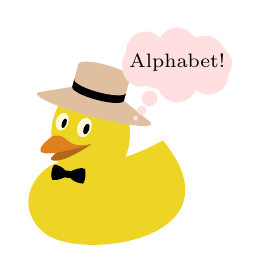
\begin{tikzpicture}
 \duck[laughing,bowtie,
strawhat=brown!50!white,
ribbon=black,
think={\scriptsize Alphabet!},
bubblecolour=white!50!pink]
\end{tikzpicture}


\end{frame}
%%%%%%%%%%%%%%%%%%%%%%%%%%%%%%%%%%
\begin{frame}[plain]{文字の数}
\Large

英語\pause
\begin{itemize}\setbeamertemplate{items}[square]
 \item アルファベットは26種類\pause
 \item 大文字と小文字があります
\end{itemize}

\pause
\mbox{}\hfill{}ということは、ぜんぶで
$26\times{}2=52$

\pause
\bigskip

いっぽう日本語は\pause

\begin{itemize}\setbeamertemplate{items}[square]
 \item ひらがな・カタカナ\pause\mbox{}\hfill{}$46\times{}2=92$\pause
 \item 漢字\pause\mbox{}\hfill{}常用漢字は2,136
\end{itemize}

\pause

\mbox{}\hfill{}ということは、ぜんぶで$92+\text{2,136}=\text{2,228}$
\end{frame}
%%%%%%%%%%%%%%%%%%%%%%%%%%%%%%%%%%%%%%%%%%%%%%
\begin{frame}[plain]{文字の数}
 \centering
 \Huge

$\text{English: 52}<\text{2,228: Japanese}$

\vfill
\normalsize

\raggedleft
\begin{tikzpicture}
\duck[tshirt,
jacket=gray,
bowtie,
crazyhair,
speech={\tiny よかった},
laughing,
signpost=\scalebox{0.4}{
\parbox{2cm}{
英語は\\
文字が\\少ない!}},
]
\end{tikzpicture}
\end{frame}
%%%%%%%%%%%%%%%%%%%%%%%%%%%%%%
\againframe<6>{what_is_alphabet}
%%%%%%%%%%%%%%%%%%%%%%%%%%%%%%%%%%%%%%%%%%%%%
\section{大文字と小文字の使いわけ}
%%%%%%%%%%%%%%%%%%%%%%%%%%%%%%%%%%%%%%%%%%%%%%
\subsection{大文字と小文字の使いわけ}

 \begin{frame}[plain]{大文字と小文字の使いわけ}
 \Large
\begin{rmfamily}

\visible<1->{\alt<2->{\textcolor{NavyBlue}{\textbf S}}{S}he is very kind.}\hfill\visible<2->{{\small 文の先頭}}

\visible<3->{\alt<4->{\textcolor{NavyBlue}{\textbf C}}{C}an \alt<5->{\textcolor{BurntOrange}{\textbf I}}{I} help you?}\hfill\visible<5->{{\small Iはいつでも}}

\visible<6->{\alt<7->{\textcolor{NavyBlue}{\textbf M}}{M}y name is \alt<8->{\textcolor{Maroon}{\textbf G}}{G}eorge \alt<8->{\textcolor{Maroon}{\textbf S}}{S}mith.}\pause\hfill{}\visible<8->{{\small 人の名前}}

\visible<9->{\alt<10->{\textcolor{NavyBlue}{\textbf H}}{H}e lives in \alt<11->{\textcolor{Maroon}{\textbf B}}{B}oston, \alt<11->{\textcolor{Maroon}{\textbf M}}{M}assachusetts.}\pause\hfill{}\visible<11->{{\small 地名}}


\end{rmfamily}

\begin{block}<12->{Topics for Today}\small
つぎのときは大文字をつかいすまj
\begin{itemize}\setbeamertemplate{items}[square]
 \item 文の先頭
 \item I(わたしは)
 \item 人の名前、地名
\end{itemize}
 \end{block}

\end{frame}
%%%%%%%%%%%%%%%%%%%%%%%%%%%%%%
\begin{frame}[plain]{動画視聴}
\LARGE

動画視聴
\end{frame}
%%%%%%%%%%%%%%%%%%%%%%%%%%%%%%%%%%%%%%%%%%%%%%
\subsection{大文字}
\begin{frame}[plain,label=upper]{アルファベット(大文字)}
\Huge
\begin{rmfamily}\bfseries
\setbeamercovered{transparent}
\begin{tabular}{cccccccccc}
\onslide<2,28,29,55->{A}&
\onslide<3,28,30,55->{B}&
\onslide<4,28,31,55->{C}&
\onslide<5,28,32,55->{D}&
\onslide<6,28,33,55->{E}&
\onslide<7,28,34,55->{F}&
\onslide<8,28,35,55->{G}&
\onslide<9,28,36,55->{H}&
\onslide<10,28,37,55->{I}&
\onslide<11,28,38,55->{J} \\
\onslide<12,28,39,55->{K}&
\onslide<13,28,40,55->{L}&
\onslide<14,28,41,55->{M}&
\onslide<15,28,42,55->{N}&
\onslide<16,28,43,55->{O}&
\onslide<17,28,44,55->{P}&
\onslide<18,28,45,55->{Q}&
\onslide<19,28,46,55->{R}&
\onslide<20,28,47,55->{S}&
\onslide<21,28,48,55->{T}\\
\onslide<22,28,49,55->{U}&
\onslide<23,28,50,55->{V}&
\onslide<24,28,51,55->{W}&
\onslide<25,28,52,55->{X}&
\onslide<26,28,53,55->{Y}&
\onslide<27,28,54,55->{Z}&
 & & &  \\
\end{tabular}
\end{rmfamily}

\mbox{}\hfill{}{\scriptsize \myaudio{./audio/001_alphabet_01.mp3}}
\end{frame}
%%%%%%%%%%%%%%%%%%%%%%%%%%%%%%%%%%
%\againframe{upper}
%%%%%%%%%%%%%%%%%%%%%%%%%%%%%%%%%%%%%%%%%%%%%%
\subsection{小文字}
\begin{frame}[plain,label=lower]{アルファベット(小文字)}
\Huge
\begin{rmfamily}\bfseries
\setbeamercovered{transparent}
\begin{tabular}{cccccccccc}
\onslide<2,28,29,55->{a}&
\onslide<3,28,30,55->{b}&
\onslide<4,28,31,55->{c}&
\onslide<5,28,32,55->{d}&
\onslide<6,28,33,55->{e}&
\onslide<7,28,34,55->{f}&
\onslide<8,28,35,55->{\rotatebox{12.5}{\itshape g}}&
\onslide<9,28,36,55->{h}&
\onslide<10,28,37,55->{i}&
\onslide<11,28,38,55->{j} \\
\onslide<12,28,39,55->{k}&
\onslide<13,28,40,55->{l}&
\onslide<14,28,41,55->{m}&
\onslide<15,28,42,55->{n}&
\onslide<16,28,43,55->{o}&
\onslide<17,28,44,55->{p}&
\onslide<18,28,45,55->{q}&
\onslide<19,28,46,55->{r}&
\onslide<20,28,47,55->{s}&
\onslide<21,28,48,55->{t}\\
\onslide<22,28,49,55->{u}&
\onslide<23,28,50,55->{v}&
\onslide<24,28,51,55->{w}&
\onslide<25,28,52,55->{x}&
\onslide<26,28,53,55->{y}&
\onslide<27,28,54,55->{z}&
 & & &  \\
\end{tabular}
\end{rmfamily}

\mbox{}\hfill{}{\scriptsize \myaudio{./audio/001_alphabet_01.mp3}}
\end{frame}
%%%%%%%%%%%%%%%%%%%%%%%%%%%%%%
\subsection{まとめ}
\begin{frame}[plain,label=matome]{まとめ}
  \begin{block}{Topics for Today}
\small
\pause
\begin{itemize}\setbeamertemplate{items}[square]
 \item アルファベットは26種類です\pause
 \item 大文字と小文字があります\pause
       \begin{itemize}
	\item 大文字小文字を区別して書けるようになろう\pause
        \item 大文字を使うのは\pause
              \begin{itemize}
	       \item 文の先頭\pause
	       \item \textrm{I}\,\,(わたし)はいつでも\pause
	       \item 人名、地名\pause
	      \end{itemize}
       \end{itemize}
 \item 聞き取れるようになったら実際に発音してみよう
\end{itemize}
      \end{block}
\end{frame}
%%%%%%%%%%%%%%%%%%%%%%%%%%%%%
%\againframe{title}
%\againframe{matome}
%%%%%%%%%%%%%%%%%%%%%%%%%%%%%
\section{演習}
\begin{frame}[plain]{アルファベットを書いてみよう}

\Large

ノートにアルファベットを書いてみよう

 \end{frame}
\begin{frame}[plain]{アルファベットを書いてみよう}
\Large

まず大文字

大文字をノートに書こう

\bigskip

\begin{rmfamily}
\begin{tabular}{p{.95\textwidth}}
ABCDEFGHIJKLMNOPQRSTUVWXYZ\\
%小文字:& a b c d e f g h i j k l m n o p q r s t u v w x y z
\end{tabular}
\end{rmfamily}
\end{frame}
%%%%%%%%%%%%%%%%%%%%%%%%%%%%%%%%
\begin{frame}[plain,label=write_lower]{アルファベットを書いてみよう}
\Large

小文字をノートに書こう

\bigskip
\begin{rmfamily}
\begin{tabular}{p{.95\textwidth}}
%ABCDEFGHIJKLMNOPQRSTUVWXYZ\\
a b c d e f \rotatebox{12.5}{{\itshape g}} h i j k l m n o p q r s t u v w x y z
\end{tabular}
\end{rmfamily}\pause

\bigskip

あ、でもその前に
\end{frame}
%%%%%%%%%%%%%%%%%%%%%%%%%%%%%
\begin{frame}[plain]{まぎらわしいもの}
\Huge

\begin{columns}
\begin{column}{.3\textwidth}
\end{column}
\begin{column}{.35\textwidth}
\setbeamercovered{transparent}
\begin{itemize}[<+->]
 \item b{\LARGE と}d
 \item p{\LARGE と}q
 \item h{\LARGE と}n
 \item i{\LARGE と}j
 \item u{\LARGE と}v
\end{itemize}
\end{column}
\begin{column}{.3\textwidth}
\end{column}
\end{columns}
\end{frame}
%%%%%%%%%%%%%%%%%%%%%%%%%%%%
\begin{frame}[plain]{まぎらわしいもの}
 
 \Huge
\centering

\scalebox{2}{%
b{\large と}d%
}
\end{frame}
%%%%%%%%%%%%%%%%%%%%%%%%%%%%
\begin{frame}[plain]{まぎらわしいもの}
 
 \Huge
\centering

\scalebox{2}{%
\tikzmark{left_eye}bcd\tikzmark{right_eye}%
}

\begin{tikzpicture}[remember picture,overlay]
 \draw[fill=black] ([xshift=16pt,yshift=10pt]pic cs:left_eye) circle (.1);
 \draw[fill=black] ([xshift=25pt,yshift=10pt]pic cs:right_eye) circle (.1);
\end{tikzpicture}
\end{frame}
%%%%%%%%%%%%%%%%%%%%%%%%%%%%
\begin{frame}[plain]{まぎらわしいもの}
 
 \Huge
\centering

\scalebox{2}{%
p{\large と}q%
}
\end{frame}
%%%%%%%%%%%%%%%%%%%%%%%%%%%%
\begin{frame}[plain]{まぎらわしいもの}
 
 \Huge
\centering

\scalebox{2}{%
b{\large と}d{\large と}p{\large と}q%
}
\end{frame}
%%%%%%%%%%%%%%%%%%%%%%%%%%%%
\begin{frame}[plain]{まぎらわしいもの}
 
 \Huge
\centering

\scalebox{2}{%
h{\large と}n%
}
\end{frame}
%%%%%%%%%%%%%%%%%%%%%%%%%%%%
\begin{frame}[plain]{まぎらわしいもの}
 
 \Huge
\centering

\scalebox{2}{%
i{\large と}j%
}
\end{frame}
%%%%%%%%%%%%%%%%%%%%%%%%%%%%
\begin{frame}[plain]{まぎらわしいもの}
 
 \Huge
\centering

\scalebox{2}{%
u{\large と}v%
}
\end{frame}
%%%%%%%%%%%%%%%%%%%%%%%%%%%%
\againframe<1>{write_lower}
%%%%%%%%%%%%%%%%%%%%%%%%%%%%%
%\againframe<1>{upper}
%\againframe<1>{lower}
%%%%%%%%%%%%%%%%%%%%%%%%%%%%
\begin{frame}[plain]{Quiz 1}
 \large
\visible<1->{%
これからアルファベットを読みあげます。

聞こえたアルファベットを順番に小文字で書いてください。
}
\mbox{}\hfill\visible<1->{{\scriptsize \myaudio{./audio/001_alphabet_011.mp3}}}

\bigskip

\begin{tabular}{rl}
1&\visible<2->{apple}\\
2&\visible<3->{bag}\\
3&\visible<4->{cat}\\
4& \visible<5->{dog}\\
5&\visible<6->{egg}
\end{tabular}

\mbox{}\hfill\visible<1->{{\scriptsize \myaudio{./audio/001_alphabet_012.mp3}}}

\end{frame}
%%%%%%%%%%%%%%%%%%%%%%%%%%%%
\begin{frame}[plain]{Quiz 2}
 \large
これからアルファベットを読みあげます。

聞こえたアルファベットを順番に大文字で書いてください。

ぜんぶで10文字です。

音声は2回繰り返します。


\mbox{}\hfill{\scriptsize {\myaudio{./audio/001_alphabet_02.mp3}}}

\end{frame}
%%%%%%%%%%%%%%%%%%%%%%%%%%%%%%
\begin{frame}[plain]{Answer}
 \Huge
 \centering
E\pause{}D\pause{}U\pause{}O\pause{}P\pause{}\,\,
C\pause{}H\pause{}I\pause{}B\pause{}A
\end{frame}
%%%%%%%%%%%%%%%%%%%%%%%%%%%%%%%
\begin{frame}{}
\Huge

\centering

English is fun.
\end{frame}

\section*{See you next time.}
%\begin{frame}{}
%\phantomsection
%\end{frame}
\end{document}
